%%*****************************************************************************
\SVN$Id$
%%*****************************************************************************
%%
%% Copyright (C) 2005-2010 The ExTeX Group and individual authors listed below
%%
%% This library is free software; you can redistribute it and/or modify it
%% under the terms of the GNU Lesser General Public License as published by the
%% Free Software Foundation; either version 2.1 of the License, or (at your
%% option) any later version.
%%
%% This library is distributed in the hope that it will be useful, but WITHOUT
%% ANY WARRANTY; without even the implied warranty of MERCHANTABILITY or
%% FITNESS FOR A PARTICULAR PURPOSE. See the GNU Lesser General Public License
%% for more details.
%%
%% You should have received a copy of the GNU Lesser General Public License
%% along with this library; if not, write to the Free Software Foundation,
%% Inc., 59 Temple Place, Suite 330, Boston, MA 02111-1307 USA
%%
%%*****************************************************************************
%% @author Gerd Neugebauer
%% @author Michael Niedermair
%%-----------------------------------------------------------------------------
\section{Eclipse}\index{Eclipse|(}

\index{Helios|see{Eclipse $\rightarrow$ Helios}}%
\index{Subversion|seealso{Eclipse $\rightarrow$ Plugins $\rightarrow$ Subversive}}%
\index{Eclipse!Plugins!Subversive|seealso{Subversion}}%
\index{Checkstlye|seealso{Eclipse $\rightarrow$ Plugins $\rightarrow$ Checkstyle}}%
\index{FindBugs|seealso{Eclipse $\rightarrow$ Plugins $\rightarrow$ FindBugs}}%
%\index{}%
Eclipse (\url{http://www.eclipse.org}) is a free IDE for Java and
other programming languages. It also provides a framework for the
development of own programs. But this is not needed for the \ExTeX\ 
core. Currently the version 3.6 (Helios\index{Eclipse!Helios}) of
Eclipse is used within the \ExTeX\ development team.
\begin{figure}[h]
  \centering  
\includegraphics[scale=.5]{image/eclipse/splash}
  \caption{The Eclipse Splash Screen}\index{Eclipse!splash screen}\label{fig:eclipse}
\end{figure}

\subsection{Eclipse Installation}

Eclipse can be downloaded for free from \url{http://www.eclipse.org}.
There you can get a file appropriate for your operating system
containing the software development kit (SDK). For instance
\begin{description}
\item [eclipse-SDK-3.6-win32.zip]\ \\
  for any decent \+Windows+ platform.
\item [eclipse-SDK-3.6-linux-gtk.tar.gz]\ \\
  for \+Linux+ on Intel x86 (32 bit) with GTK.
\end{description}

Note that we use and show here the classic
edition\index{Eclipse!classic edition} of eclipse. Other editions will
also work but show a slightly different appearance.

Download the appropriate file and unpack it in the installation
directory. A new subdirectory \Dir{eclipse} will be created
containing all files of Eclipse. You are done with the basic
installation. You can start the \File{eclipse} executable found in
the just installed directory.

\begin{figure}[ht]
  \centering  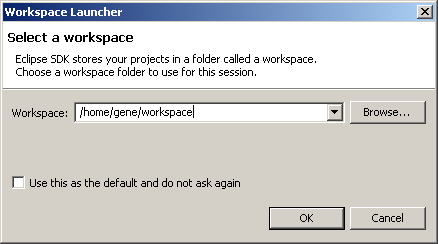
\includegraphics[scale=.5]{image/eclipse/workspace}
  \caption{\+Eclipse Workspace+}\label{fig:eclipse-workspace}
\end{figure}
When Eclipse starts you first see the splash
screen\index{Eclipse!splash screen} shown in figure~\ref{fig:eclipse}.
Then Eclipse requests a workspace -- as shown in
figure~\ref{fig:eclipse-workspace}. The
workspace\index{Eclipse!workspace} is a directory where the projects
live and where your preferences are stored. If you have chosen the
workspace directory carefully, you can turn on the check mark in this
dialog to be not asked again.

Note it is a good practice to have a separate workspace for \ExTeX{}
and not mix it with other Eclipse projects. \ExTeX{} comes with a
multitude of Eclipse projects itself. Thus other project might get
lost in the workspace.

Finally you end up in the welcome window of Eclipse shown in
figure~\ref{fig:eclipse-welcome}. Take some time and read the
introductory material found there.
\begin{figure}[ht]
  \centering  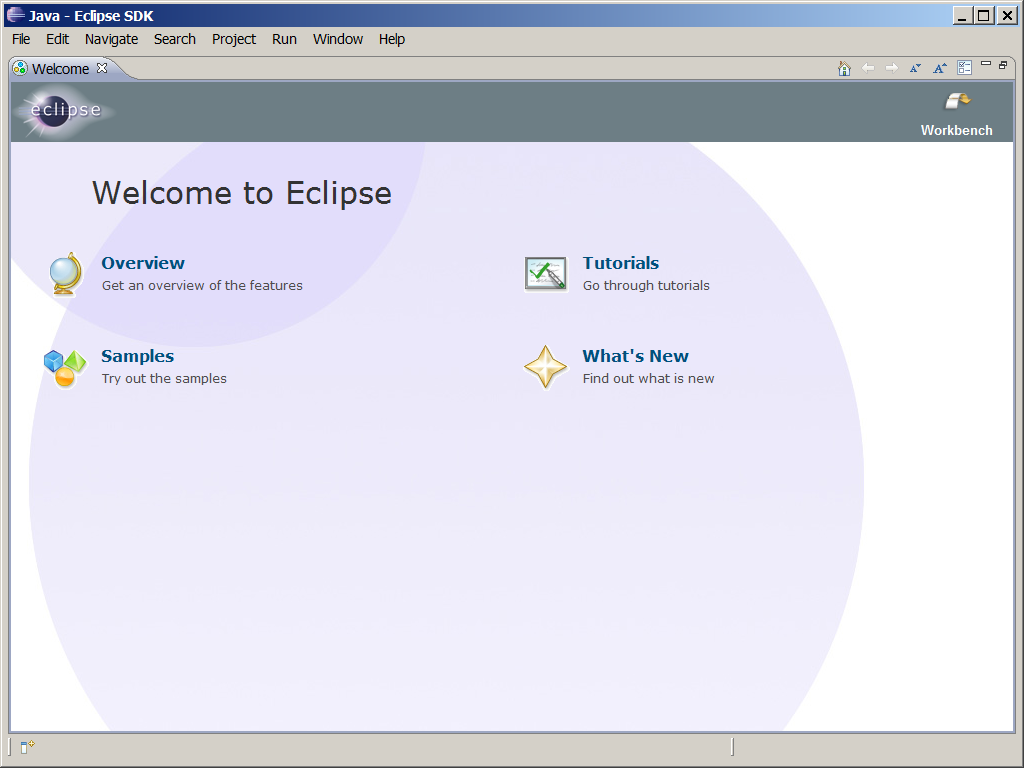
\includegraphics[scale=.33]{image/eclipse/welcome}
  \caption{Eclipse Initial Window}\label{fig:eclipse-welcome}
\end{figure}

The following sections describe some of the configurations which
should be performed in order to work with Eclipse on \ExTeX.

\subsection{Configuring Eclipse}

Eclipse can be configured in a wide range. In the following sections
some configuration options are proposed for the seamless development
of \ExTeX. The configuration is performed via the preferences dialog.
This dialog can be opened via \menu{Window \sub Preferences\ldots}
\begin{figure}[htp]
  \hbox{}\hfill
  \subfloat[Eclipse Preferences\label{fig:eclipse-preferences}]{%
    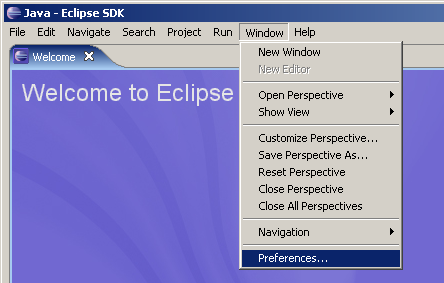
\includegraphics[scale=.4]{image/eclipse/preferences}}%
  \hfill
  \subfloat[Eclipse Print Margin\label{fig:eclipse-print-margin}]{%
    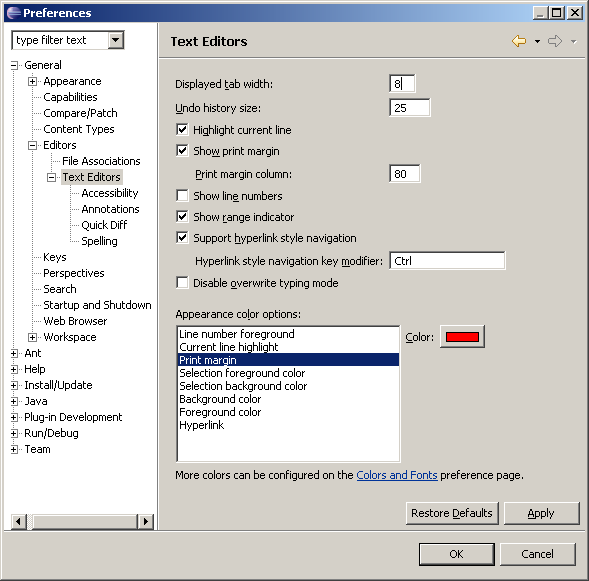
\includegraphics[scale=.4]{image/eclipse/print-margin}}%
  \caption{Some simple Settings}\index{Eclipse!print margin}
\end{figure}

This menu brings up a dialog with many tabs which can be used to
adjust the behaviour of Eclipse in many ways. The first step described
below consists of the adaption of the appearance of the text editors.
In the tree view on the left side of the dialog select \menu{General
  \sub Editors \sub Text Editors} as shown in
figure~\ref{fig:eclipse-print-margin}.

Now you can adjust some values on the right side of the dialog. Set
the tag width to 8. Check the item \menu{Show print margin}. Adjust
the print margin to 80. And finally change the print color to red. The
settings are stored in the workspace by accepting the settings with
the \menu{OK} button.

The rational is that the tabs should be used in the traditional sense
of eight chracters wide. In fact this is just a fallback. Usually tabs
should be avoided where possible. The print margin\index{Eclipse!print
margin} of 80 is a weak
rule. Try to limit yourself to this width. Sometimes it is not
reasonable. Thus the \+Checkstyle+ rules allow some more characters
before complaining.

The following sections describe some more of the configuration
options. You should really consider to follow the instructions to make
maximal use of the configurations provided with \ExTeX.



\subsubsection{Code Templates}

Code templates provide a convenient way of filling in a frame for the
documentation whenever some code is generated by Eclipse. The \ExTeX\
repository contains in the file
\Dir*{develop/eclipse}\File{codetemplates.xml} some definitions of code
templates. To import those definitions use the preferences (see
figure~\ref{fig:eclipse-preferences}). Here select the item \menu{Java
  \sub Code Style \sub Code Templates}. The button \menu{Import\ldots}
can leads to a file selector where the file
\Dir*{develop/eclipse}\File{codetemplates.xml} should be entered.
\begin{figure}[htp]
  \centering  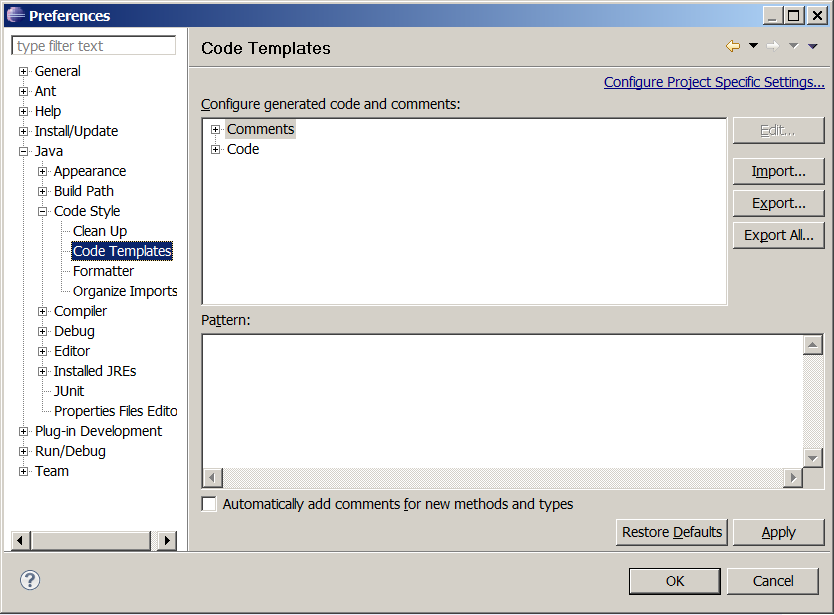
\includegraphics[scale=.4]{image/eclipse/templates}
  \caption{Eclipse Preferences}\label{fig:eclipse-templates}
\end{figure}

After the code templates have been loaded a minor adaption is
required. The entry under the key \menu{Comments \sub Types} containes
hard-wired a name and email address of the author. Here the own name
and email address should be entered (see
figure~{fig:eclipse-template-author}).
\begin{figure}[htp]
  \centering  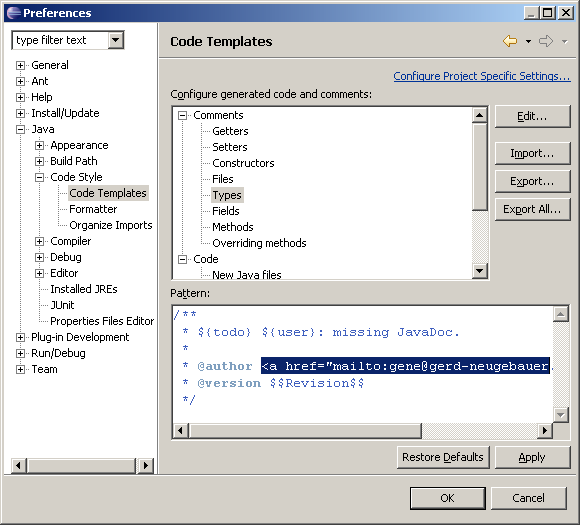
\includegraphics[scale=.4]{image/eclipse/template-author}
  \caption{Code Template Author Name}\label{fig:eclipse-template-author}
\end{figure}


\subsubsection{The Code Formatter}

Eclipse comes has a code formatter which can be invoked easily. This
code formatter can be configured for different needs. A configuration
for \ExTeX\ is contained in the repository under
\texttt{develop/eclipse/formatter.xml}. In Eclipse the preference page
can be found under the key \menu{Java \sub Code Style \sub Formatter}.
ere you can use the button \menu{Import\dots} and select the
configuration file. Now the profile ``gene'' is loaded and can be
selected. This is shown in figure~\ref{fig:eclipse-formatter-gene}.
\begin{figure}[htp]
  \centering  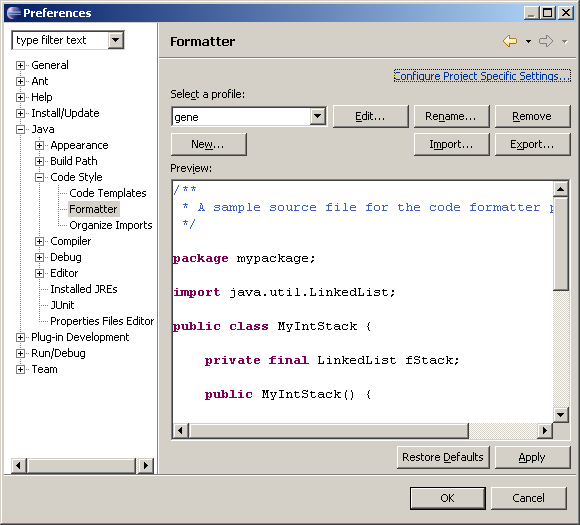
\includegraphics[scale=.4]{image/eclipse/formatter-gene}
  \caption{Settings for the Code Formatter}\label{fig:eclipse-formatter-gene}
\end{figure}

The formatter for Ant files has distinct parameters which should be
adapted. The preference page can be found under the key \menu{Ant \sub
  Editor \sub Formatter}. The values should be adjusted as shown in
figure~\ref{fig:eclipse-ant-formatter}.
\begin{figure}[htp]
  \centering  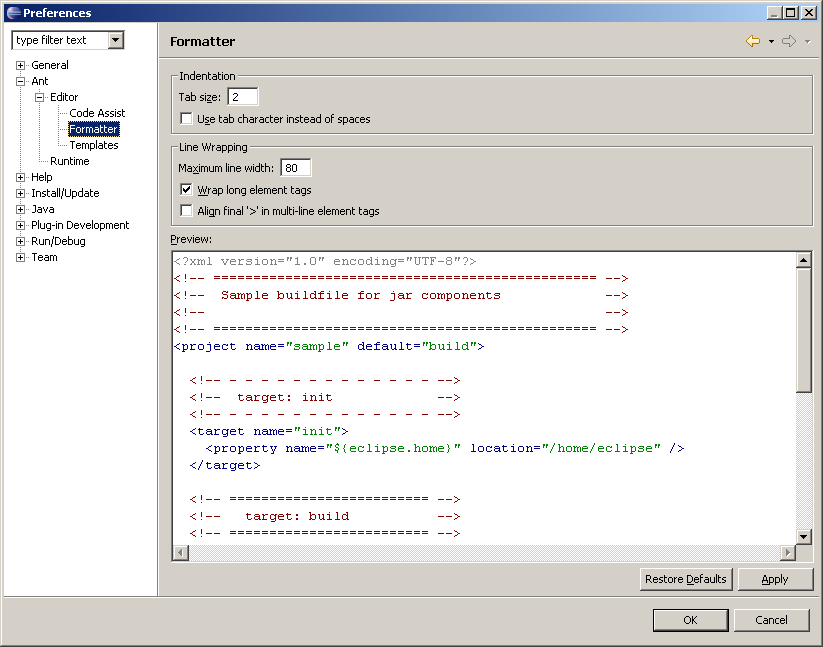
\includegraphics[scale=.4]{image/eclipse/ant-formatter}
  \caption{Settings for the Ant Formatter}\label{fig:eclipse-ant-formatter}
\end{figure}


\subsubsection{Spelling}\index{spell checker|(}

Since English is not the native language of each developer it is a
good idea to enable the spell checking of the source code. This
feature is provided by Eclipse. In figure~ref{fig:eclipse-spelling}
you can seen the preference page where you can activate the spell
checking and provide a dictionary.
\begin{figure}[htp]
  \centering
  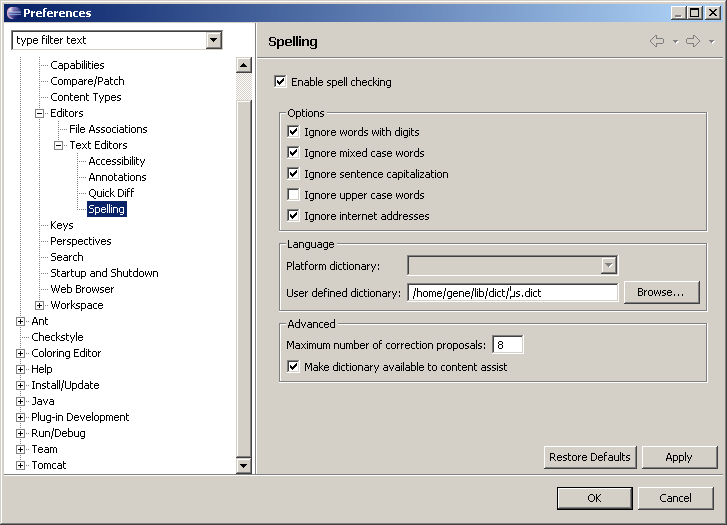
\includegraphics[scale=.4]{image/spelling}
  \caption{Spelling Preferences}\label{fig:eclipse-spelling}
\end{figure}

A dictionary\index{dictionary} can be got from SCOWL\index{SCOWL}
(\url{http://wordlist.sourceforge.net/}). You might want to use the US
dictionary of medium size. Since this contains enough words to fit but
not too much obscure words which hide typos.

After the spell checking is activated potential typos are marked in
the editor with yellow lines. Correction proposals can be requested
with the quick fix shortcut Ctrl-1.
\index{spell checker|)}


\subsubsection{Maven}\index{Maven|(}

To prepare the interaction with Maven you need to define the classpath
variable \texttt{M2\_REPO}. This is done with the help of a Maven
task:
\begin{lstlisting}{}
# mvn -Declipse.workspace=. eclipse:configure-workspace
\end{lstlisting}
This command should be issued in a shell when the current directory is
the Eclipse workspace directory. Alternatively you can give an
absolute or relative path to the workspace directory instead of the
\File{.} in the define.

You can control that the plugin did the right thing. In the
preferences dialog check the list under \menu{Java \sub Build Path
  \sub Classpath Variables}. It should now (maybe after a restart of
Eclipse) contain a variable \texttt{M2\_REPO} pointing to the Maven
repository.
\index{Maven|)}


\subsection{Eclipse Plugins}\label{sec:eclipse.plugins}\index{Eclipse!Plugins|(}

Eclipse can be extended with plugins which provide additional
functionality. It is recommended to use some of them.

The installation of a plugin follows the same scheme.

\begin{itemize}
\item The menu \menu{Help \sub Install New Software \ldots} (see
  figure~\ref{fig:eclipse-install-new-software}) opens the dialog for
  software installation.
\item Add or select an update site (see
  figure~\ref{fig:eclipse-install-subversive}).
\item The list is filled with the available software components from
  this site.  Mark the software components to be installed in this
  list and submit with the \textsf{Next} button.
\item Check the list for correctness and accept the licence agreements
  -- after reading and understanding.
\item Restart Eclipse when requested.
\end{itemize}
\begin{figure}[ht]
  \hbox{}\hfill
  \subfloat[Install New Software Menu\label{fig:eclipse-install-new-software}]{%
    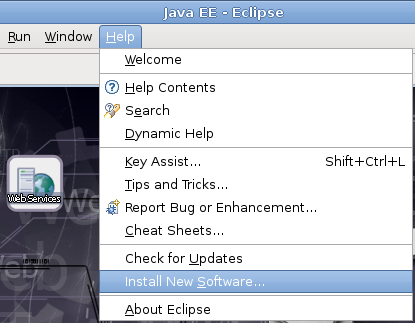
\includegraphics[scale=.4]{image/eclipse/install-new-software}}%
  \hfill
  \subfloat[The Installation Dialog
             Perspective''\label{fig:eclipse-install-subversive}]{%
    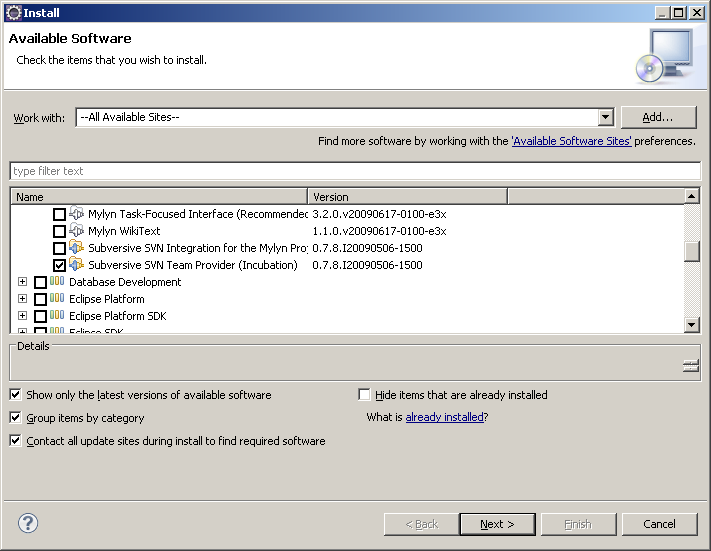
\includegraphics[scale=.4]{image/eclipse/install-subversive}}%
  \hfill\hbox{}

  \caption{Installing a Plugin}\index{Eclipse!plugin}\label{fig:eclipse-plugin}
\end{figure}

The following plugins can be considered for installation.


\subsubsection{Subversive}\index{Eclipse!Plugins!Subversive}\label{sec:subversive}
This is an integrated Subversion\index{Subversion} client to Eclipse.
\begin{description}
\item [Update site:] \url{http://download.eclipse.org/releases/galileo}
\item [Component:] \menu{Collaboration \sub Subversive SVN Team Provider}
\end{description}
You need additionally the connectors for Subclispe to connect to a Subversion
server.\index{Eclipse!Plugins!Subversive connectors}
\begin{description}
\item [Update site:] \url{http://community.polarion.com/projects/subversive/download/eclipse/2.0/galileo-site/}
\item [Component:] \menu{Subversive SVN Connectors \sub Subversive SVN Connectors}
\end{description}

This plugin is highly recommended. Alternatively the subclipse plugin
can be used for the same purpose.


\subsubsection{Checkstyle}\index{Eclipse!Plugins!Checkstyle|(}\label{sec:eclipse.checkstyle}

\+Checkstyle+ is a tool for checking the adherence of Java source code
to certain rules. The rules can be freely configured. The \ExTeX\ 
repository contains a set of rules for Checkstyle.
\begin{description}
\item [Update site:] \url{http://eclipse-cs.sf.net/update/}
\item [Component:] \menu{Eclipse Checkstyle Plug-in \sub Eclipse
    Checkstyle Plug-in 5.0.1}\\
  or any decent version
\end{description}
This plugin is highly recommended.

To set the configuration use \menu{Window \sub Preferences \sub Checkstyle}.
Create a new configuration and set the values in
figure~\ref{fig:eclipse-checkstyle-config}.

The configuration is stored in \Dir*{develop/eclipse}\File{extex\_checkstyle.xml}.
\begin{figure}[htp]
  \centering  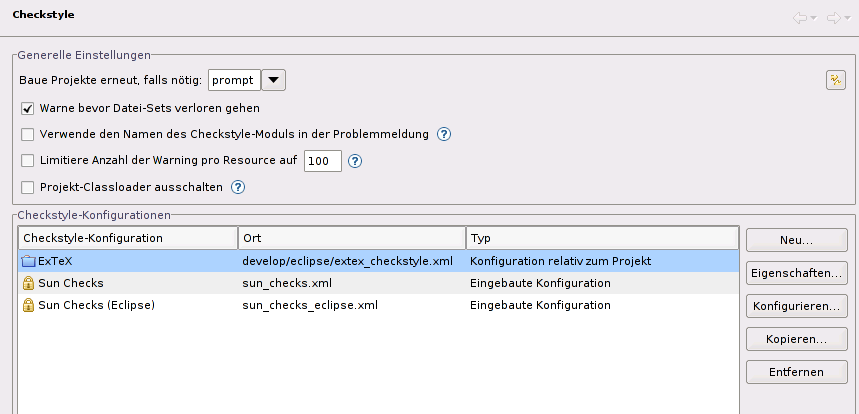
\includegraphics[scale=.5]{image/eclipse/checkstyle-config}
  \caption{Checkstyle configuration}\label{fig:eclipse-checkstyle-config}
\end{figure}

To enable the checks set in \menu{Project \sub Properties \sub
  Checkstyle} the configuration to \emph{ExTeX} (see
figure~\ref{fig:eclipse-checkstyle-enable}).
\begin{figure}[htp]
  \centering  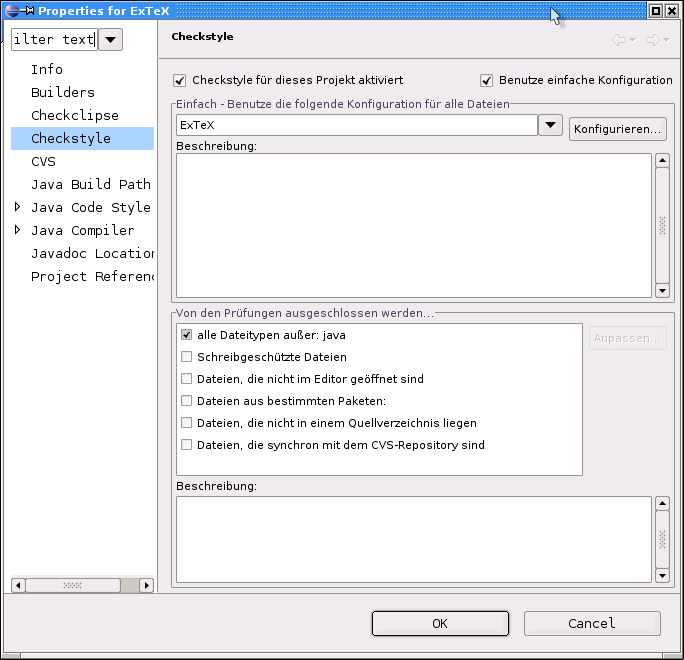
\includegraphics[scale=.5]{image/eclipse/checkstyle-enable}
  \caption{enable Checkstyle}\label{fig:eclipse-checkstyle-enable}
\end{figure}
\index{Eclipse!Plugins!Checkstyle|)}

\subsubsection{FindBugs}\index{Eclipse!Plugins!FindBugs}
This is an integration of the \+FindBugs+ analyzer to detect code
anomalies in Eclipse.
\begin{description}
\item [Update site:] \url{http://findbugs.cs.umd.edu/eclipse}
\item [Component:] \menu{FindBugs}
\end{description}
This plugin is highly recommended.


\subsubsection{EclEmma}\index{Eclipse!Plugins!EclEmma|(}\index{EclEmma}
This is an integration of the code coverage tool \+Emma+ into
Eclipse.
\begin{description}
\item [Update site:] \url{http://update.eclemma.org/}
\item [Component:] \menu{EclEmma}
\end{description}
This plugin is recommended.
\index{Eclipse!Plugins!EclEmma|)}


\subsubsection{TeXlipse}\index{Eclipse!Plugins!TeXlipse|(}\index{TeXlipse}
This plugin provides tools and editors for dealing with \LaTeX\ 
documents in Eclipse.
\begin{description}
\item [Update site:] \url{http://texlipse.sourceforge.net/}
\item [Component:] \menu{TeXlipse}
\end{description}
This plugin is optional.
\index{Eclipse!Plugins!TeXlipse|)}


\subsubsection{EPIC}\index{Eclipse!Plugins!EPIC}
This is a set of tools and editors to deal with \+Perl+
programs in Eclipse in Eclipse.
\begin{description}
\item [Update site:] \url{http://e-p-i-c.sf.net/updates}
\item [Component:] \menu{EPIC Main Components \sub EPIC}
\end{description}
This plugin is recommended if you are interested in the few parts
written in \+Perl+.


\subsubsection{Wicked Shell}\index{Eclipse!Plugins!Wicked Shell|(}\index{shell}
This plugin provides means to run shells inside Elipse.
\begin{description}
\item [Update site:] \url{http://www.wickedshell.net/updatesite}
\item [Component:] \menu{Wicked Shell}
\end{description}
This plugin is optional.
\index{Eclipse!Plugins!Wicked Shell|)}
%
\index{Eclipse!Plugins|)}


\subsection{Getting Started}

\subsubsection{Downloading the Sources}

Now we are ready to create a project for the sources of \ExTeX.
Everything needed can be found in the Subversion repository of \ExTeX\ 
hosted by \+Berlios+. Thus we start to get things onto the local host.
For this purpose we need to open a new perspective in Eclipse. A
perspective is a collection of windows which are usually meant for a
common task.

A new perspective\index{Eclipse!perspective} can be opened via the
window \menu{Window \sub Open Perspective \sub Other\ldots} which can
be seen in figure~\ref{fig:eclipse-open-perspective-other}. This menu
item opens a dialog box which offers some perspectives for opening.
Currently we need a ``Subversion Exploring'' perspective. This
perspective is meant for inspecting Subversion repositories and
manipulation. Thus this perspective is selected (see
figure~\ref{fig:eclipse-select-svn}) and the dialog is completed with
the OK button.
\begin{figure}[ht]
  \hbox{}\hfill
  \subfloat[Open Perspective\label{fig:eclipse-open-perspective-other}]{%
    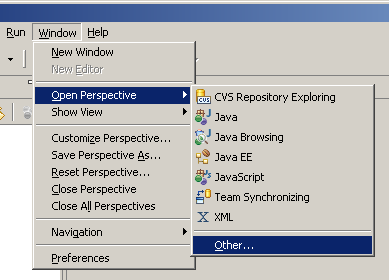
\includegraphics[scale=.4]{image/eclipse/open-perspective-other}}%
  \hfill
  \subfloat[Selecting ``Subversion Exploring
             Perspective''\label{fig:eclipse-select-svn}]{%
    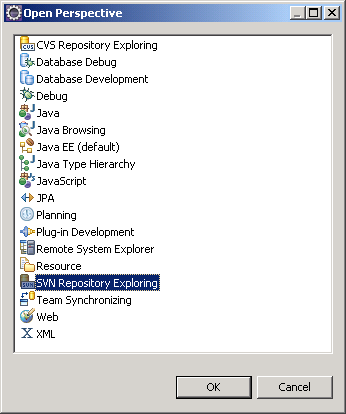
\includegraphics[scale=.4]{image/eclipse/select-svn}}%
  \hfill\hbox{}

  \caption{Switching to a Perspective}\index{Eclipse!perspective}\label{fig:eclipse-perspective}
\end{figure}

Now a Subversion exploring perspective is opened (see
figure~\ref{fig:eclipse-svn-perspective}). You see a lot of windows
and icons there. The tab ``SVN Repositories'' on the left side shows
all repository locations currently known. This list is empty since we
have not added any Subversion location yet.
\begin{figure}[ht]
  \centering  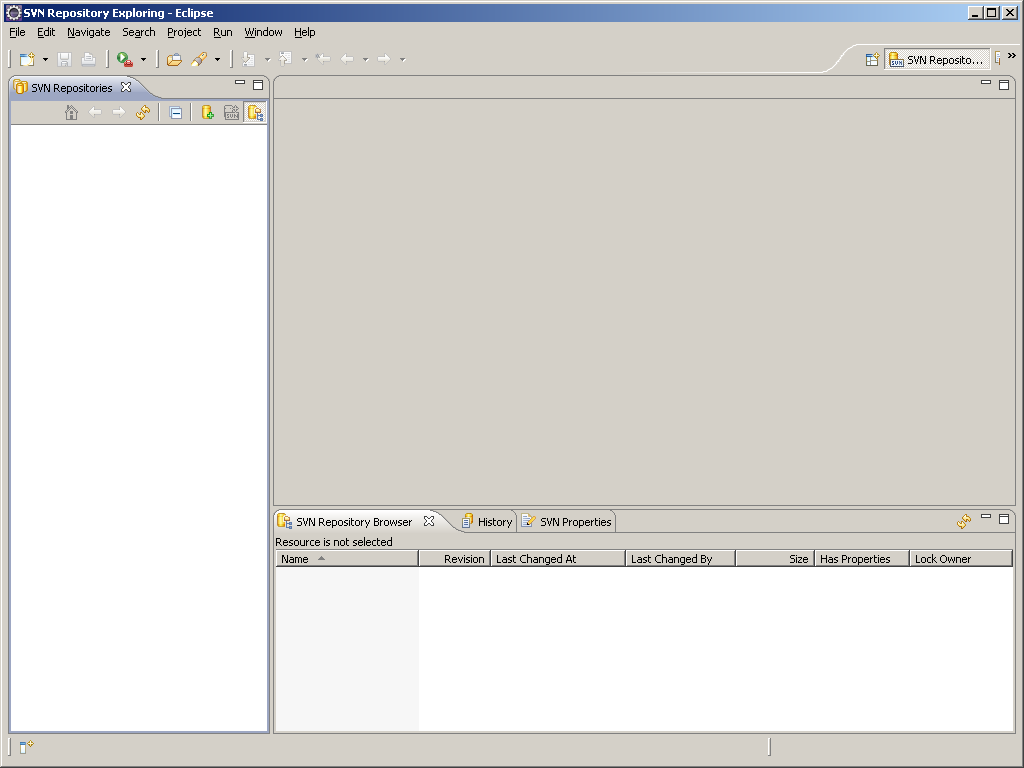
\includegraphics[scale=.33]{image/eclipse/svn-exploring}
  \caption{SVN Exploring Perspective}\label{fig:eclipse-svn-perspective}
\end{figure}

To add a new repository location press the left mouse button on this
tab and select \menu{New \sub Repository Location\ldots} (see
figure~\ref{fig:eclipse-new-repository}). This brings up the dialog
shown in figure~\ref{fig:eclipse-add-svn}. Here you can enter the
coordinates of the \ExTeX\ Subversion repository.
\begin{figure}[ht]
  \hbox{}\hfill
  \subfloat[New Repository Location\label{fig:eclipse-new-repository}]{%
    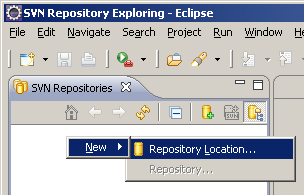
\includegraphics[scale=.4]{image/eclipse/new-repository}}%
  \hfill
  \subfloat[The Coordinates of the \ExTeX\ Subversion
  Repository\label{fig:eclipse-add-svn}]{%
    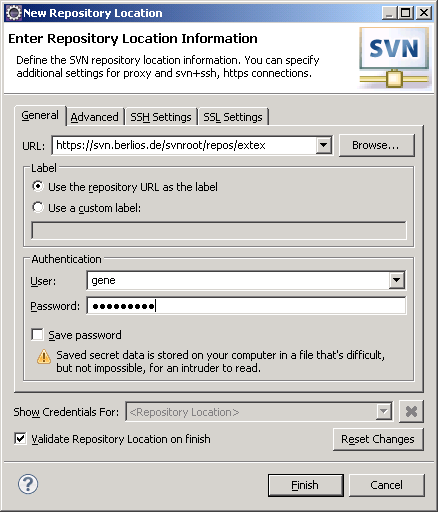
\includegraphics[scale=.4]{image/eclipse/add-svn}}%
  \caption{Adding the \ExTeX\ SVN Repository}
\end{figure}

Note that you have to enter your account at \+Berlios+ and its
password into the appropriate fields. If you do not have an account
you can use the account name \texttt{anonymous} without any password
to get reading access to the sources.

For this step you need online access to the internet. When the form is
submitted with the \textsf{OK} button, the accessibility of the
repository location is checked. Upon success the new repository
location is added to the list of repository locations as can be seen
in figure~\ref{fig:eclipse-svn}.
\begin{figure}[htbp]
  \hbox{}\hfill
  \subfloat[The \ExTeX\ Repository Listed\label{fig:eclipse-svn}]{%
    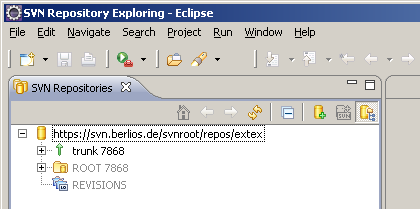
\includegraphics[scale=.4]{image/eclipse/svn}}%
  \hfill
  \subfloat[Selecting to check-out of
  \ExTeX\label{fig:eclipse-checkout-extex}]{%
    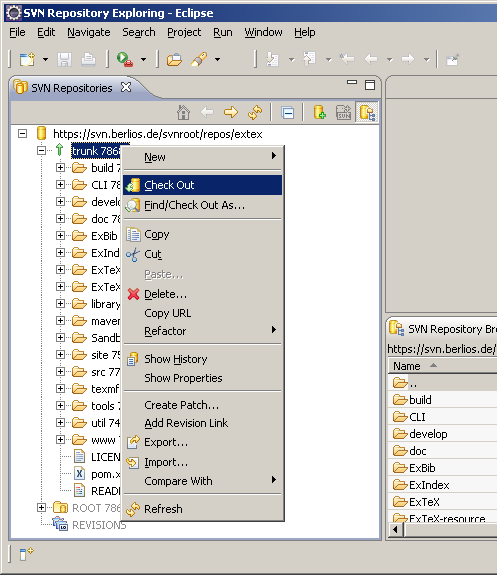
\includegraphics[scale=.4]{image/eclipse/checkout-extex}}%
  \caption{Checking-out of \ExTeX}
\end{figure}

The next step consists of the \+check-out+ of the sources into an Eclipse
project. This project serves as a first container and will not really
be used later on. To accomplish this you have to open the repository
location and the \texttt{trunk}\index{trunk|tt} within. Right-click
the item \texttt{trunk} in the list (see figure~\ref{fig:eclipse-svn})
and select \menu{Check Out} in the appearing context menu (see
figure~\ref{fig:eclipse-checkout-extex}). This will instruct Exclipe
to create a new project in the workspace and fill it with the files
from the repository. The name is inherited from the last component of
the URL -- i.e. it will be named \texttt{extex}.

Eclipse shows a progress bar during the check-out (see
figure~ref{fig:eclipse-checkout}). This operation may take some time
-- we have been really busy creating files. When the checkout is
finished you will find the project \texttt{ExTeX} in Eclipse
containing the files within. The appearance of the Package View with
those files is shown in figure~\ref{fig:eclipse-extex-project}.
\begin{figure}[htp]
  \hbox{}\hfill
  \subfloat[The Checkout Progress Bar\label{fig:eclipse-checkout}]{%
    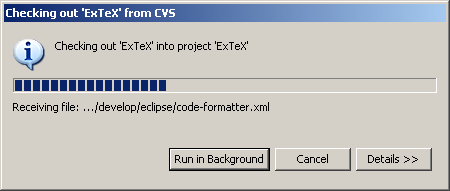
\includegraphics[scale=.4]{image/eclipse/checkout}}%
  \hfill
  \subfloat[The \ExTeX\ Project in the Package
  View\label{fig:eclipse-extex-project}]{%
    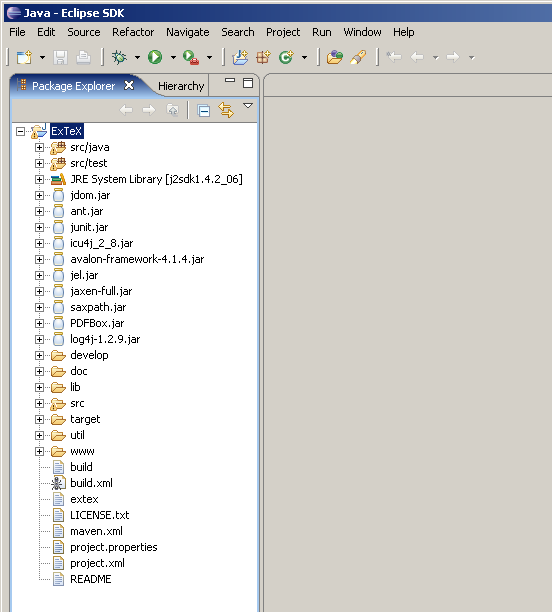
\includegraphics[scale=.4]{image/eclipse/extex-project}}%
  \caption{Checking out \ExTeX\ from the Repository}
\end{figure}

Now you should close the project in Eclipse. We will reopen the
sub-projects later on.

Alternatively you could check-out the files of \ExTeX\ externally and
open Eclipse later.


\subsubsection{Creating Eclipse Projects}

Eclipse uses some control files to define an Ecipse project. For
instance the files and diretories \File{.project}, \File{.settings},
\File{.classpath}, and \File{.checkstyle} belong to this category.
Usually these files can be generated automatically by Maven from the
information present in the pom. Thus they should not be checked into
the repository. They are included in the \+svn:ignore+ list.


\begin{lstlisting}{}
# mvn eclipse:eclipse
\end{lstlisting}

\Incomplete


\subsection{Compiling \ExTeX}

Any source file in Eclipse is compiled automatically when the file is
saved. Thus it is usually not necessary to compile things manually. If
you feel the need to recompile everything you can achieve this by
selecting \menu{Project \sub Clean\ldots} while the item \menu{Project
  \sub Build Automatically} is checked (see
figure~\ref{fig:eclipse-recompile}).
\begin{figure}[thp]
  \centering
  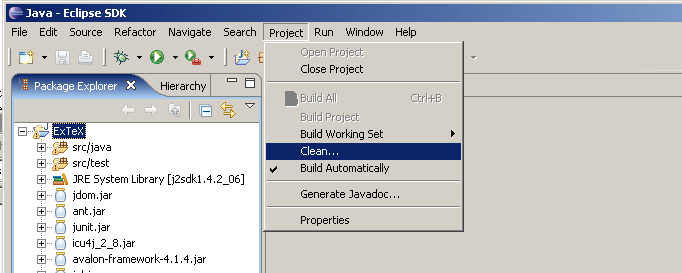
\includegraphics[scale=.4]{image/eclipse/recompile}
  \caption{Recompiling a Project}\label{fig:eclipse-recompile}
\end{figure}

Another recompilation can be triggered via the Ant task \texttt{compile}.

\subsection{Running \ExTeX}

\ExTeX\ can be run from within Eclipse. We will describe here the
execution of the compiled sources from a workspace. The executio of an
external program would be an alterative. But this is only of minor
relevance for a developer.

To run \ExTeX\ on some input file you have to create a run profile.
The profile is kept and can be used the next time again. To create a
run profile select the toolbar item \menu{Run\dots} in the Java
perspective (see figure~\ref{fig:eclipse-run-menu}). In the appearing
dialog select \menu{Java Application} and press the button \menu{New}.
Now you can fill in the tabs as seen in figure~\ref{fig:eclipse-run}.
Enter a name, the project and the main class. The main class to use is
\texttt{de.dante.extex.main.TeX}.
\begin{figure}[htp]
  \hbox{}\hfill
  \subfloat[The Run Menu\label{fig:eclipse-run-menu}]{%
    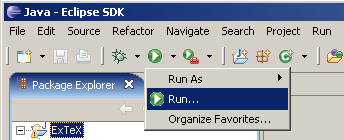
\includegraphics[scale=.4]{image/eclipse/run-menu}}%
  \hfill
  \subfloat[Creating a run configuration\label{fig:eclipse-run}]{%
    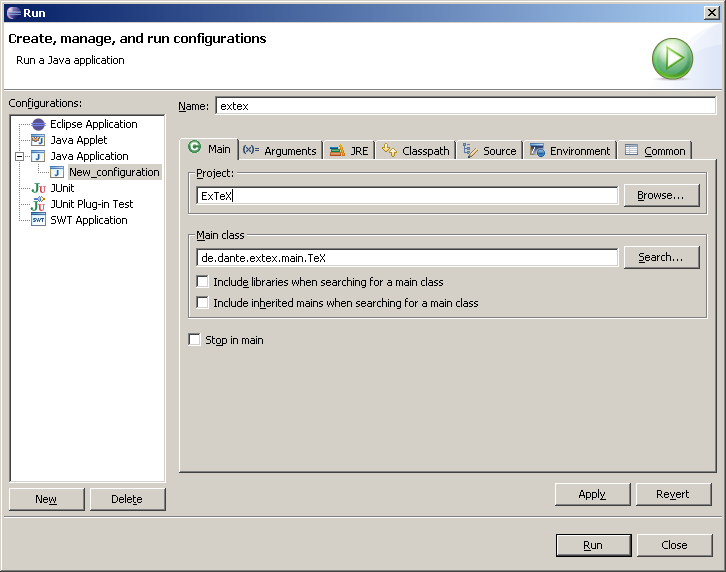
\includegraphics[scale=.4]{image/eclipse/run}}%
  \caption{Checking out \ExTeX\ from the Repository}
\end{figure}

On the \textsf{Arguments} tab you can enter the arguments for the
invocation of \ExTeX. These are the same arguments which can also be
used on the command line. Usually here the input file is given (see
figure~\ref{fig:eclipse-run-args}.
\begin{figure}[thp]
  \centering
  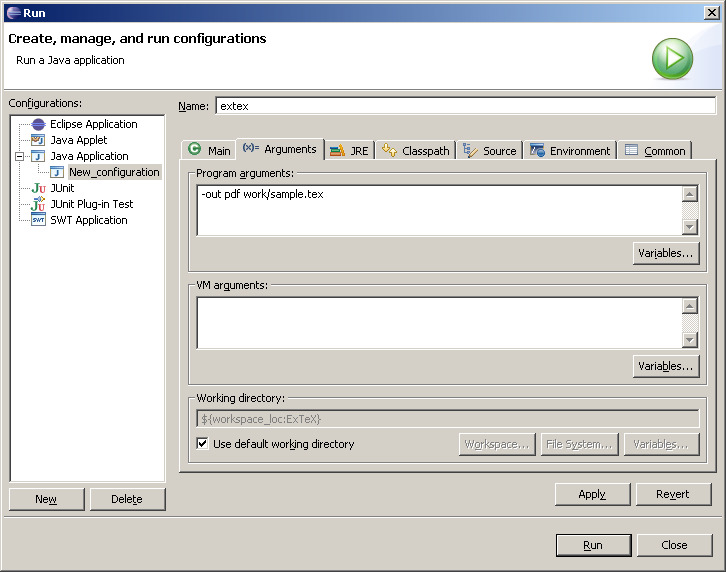
\includegraphics[scale=.4]{image/eclipse/run-args}
  \caption{Arguments for Running \ExTeX}\label{fig:eclipse-run-args}
\end{figure}

The \menu{Run} button submits the command. A Console view is opened
which can be used to interact with the the program -- like in the
command line interpreter.


\subsection{Committing Changes}

For Eclipse a Subversion plugin should be installed (see
section~\ref{sec:subversive}) which hides the details of the
underlying version control system. Thus things are quite simple for
the newcomers. On the other hand they are differnt from the procedure
on the command line or other tools whic mimic the command line (like
\+TortoiseSVN+).

The metaphor used in Eclipse is the synchronisation of the workspace
with the reporsitory. In the course of this syncronisation changes in
the workspace files are committed to the repository, changes from the
repository are updated into the workspace, and conflicts can be
resolved. The conflict resolution -- also known as merging -- is the
demanding task. Thus it has to be performed by a human.

To start the synchronisation select in the \menu{Package Manager} or
\menu{Navigator} view the topmost \ExTeX\ node and activate in the
context menu (right mouse button) the entry \menu{Team \sub Synchronize
with Repository} (see figure~\ref{fig:eclipse-team}).
\begin{figure}[htp]
  \centering
  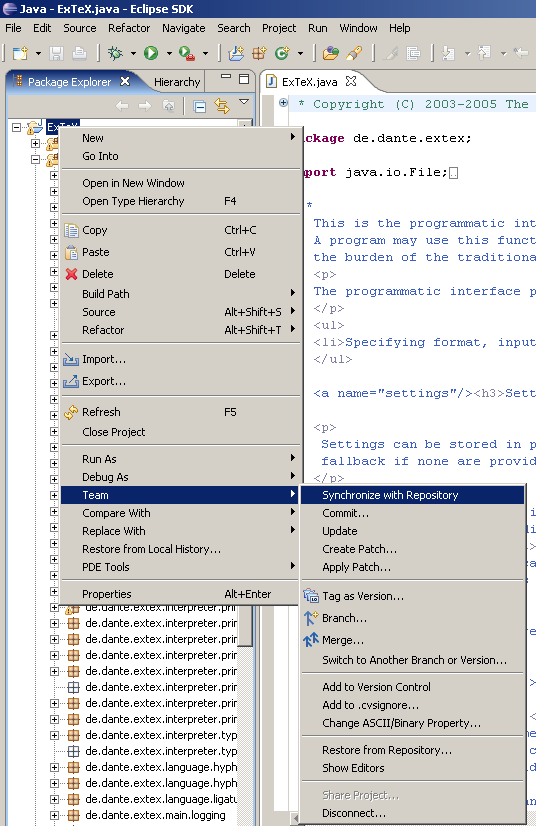
\includegraphics[scale=.4]{image/eclipse/team}
  \caption{Starting Synchronization}\label{fig:eclipse-team}
\end{figure}



\INCOMPLETE



\subsection{Running Ant from within Eclipse}\label{sec:eclipse.ant}

To use Ant from within Eclipse you have to open the Ant view. This can
be acomplished via the menu \menu{Window \sub Show View \sub Ant} (see
figure~\ref{fig:eclipse-ant-open}).

In this view use the leftmost tool to add an Ant file. In the file
selector choose the file \File{ExTeX/build.xml}. The Ant file is added
to the (previously empty) list. It can be open to show the Ant target
available (see figure~\ref{fig:eclipse-ant}).
\begin{figure}[htp]
  \hbox{}\hfill
  \subfloat[Opening an Ant View\label{fig:eclipse-ant-open}]{%
    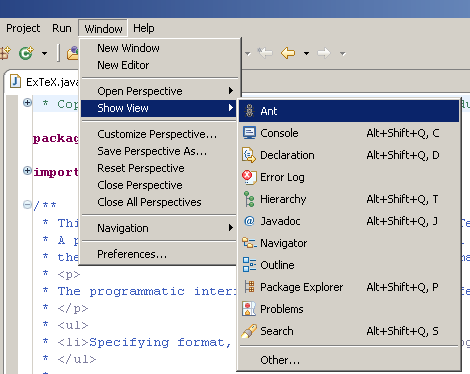
\includegraphics[scale=.4]{image/eclipse/ant-open}}%
  \hfill
  \subfloat[The Ant View for \ExTeX\label{fig:eclipse-ant}]{%
    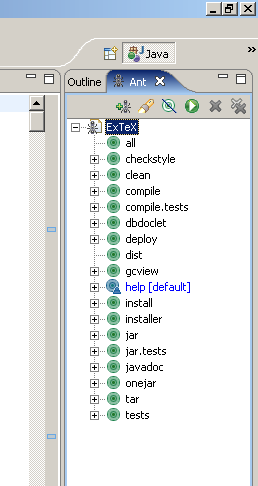
\includegraphics[scale=.4]{image/eclipse/ant}}%
  \caption{Ant in Eclipse}
\end{figure}

A double click on a target starts it's execution. The output is shown
in a Console view.

A description of the targets can be found in section~\ref{sec:Ant}.


\subsection{Creating Javadoc}

To create the \+Javadoc+ HTML description of the sources you can use
the \+Ant+ target \texttt{javadoc}. See sections \ref{sec:eclipse.ant}
and \ref{sec:Ant}. The result can be found in the directory
\Dir*{target}\Dir{javadoc}.


\subsection{Creating the Installer}

To create the installer you can use the Ant target
\texttt{installer}. See sections \ref{sec:eclipse.ant} and
\ref{sec:Ant}. The result can be found in the file
\Dir*{target}\File{ExTeX-setup.jar}.


\index{Eclipse|)}